\chapter*{Глава 9. Работа с BRAM}

\emph{Интерфейс BRAM, однопортовый и двухпортовый режимы работы.}

\section{Введение}

Внутри ПЛИС Xilinx есть специальный аппаратный ресурс – блочная память или BRAM (Block RAM). Это набор из специальных аппаратных блоков статической памяти, выполненных аппаратно, т.е. часть логики кристалла зафиксирована под память, и не может быть использована по другому назначению. Количество таких блоков зависит от конкретного типа кристалла ПЛИС и может быть до нескольких сотен. Каждый блок имеет два аппаратных порта, которые могут работать на разных тактовых частотах. 
У блочной памяти есть свои преимущества и недостатки. С одной стороны, это быстрые аппаратные блоки, способные работать на частотах до 500 МГц. При использовании блочной памяти ее разные порты могут работать на разных частотах. Это удобно использовать для синхронизации между разными клоковыми доменами. Но с другой стороны, блочная память – дорогостоящий ресурс. Количество ее ограничено. Если требуется объем памяти меньший чем объем одного блока (18 Кбит), то все равно будет использован весть блок, и неиспользованная его часть просто пропадет. 
Для создания оперативных и постоянных запоминающих устройств, реализуемых на основе блочной памяти ПЛИС, в составе генератора параметризованных модулей LogiCORE предусмотрено такое ядро, как Block Memory Generator. В данной главе будет подробно рассмотрено его использование, настройка и реализация с помощью средств языка VHDL.

\section{Создание и настройка ядра BRAM}

\subsection{Заходим в Block Memory Generator} 
Выберите Block Memory Generator из каталога IP (рис. 1-2).

\begin{figure}[H]
\centering
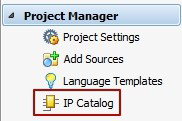
\includegraphics[width=0.6\textwidth]{1}
\caption{Рис.1}
\label{1_label}
\end{figure}

\begin{figure}[H]
\centering
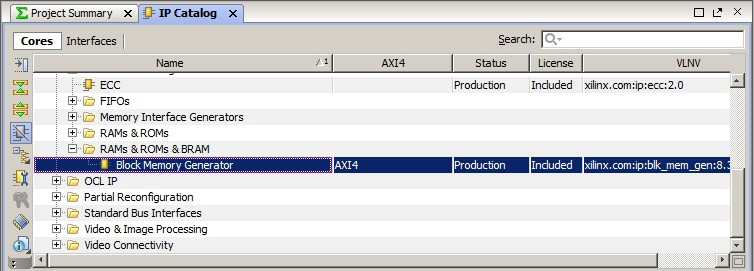
\includegraphics[width=0.6\textwidth]{2}
\caption{Рис.2}
\label{2_label}
\end{figure}

\subsection{Работа с интерфейсом BMG} 
Выбор типа и организации запоминающего устройства, формируемого на основе рассматриваемого параметризированного модуля, осуществляется с помощью соответствующего \emph {мастера} настройки параметров, который содержит от четырёх до шести (в зависимости от конфигурируемых параметров) диалоговых панелей.

\subsubsection{Basic}

\begin{figure}[h]
\centering
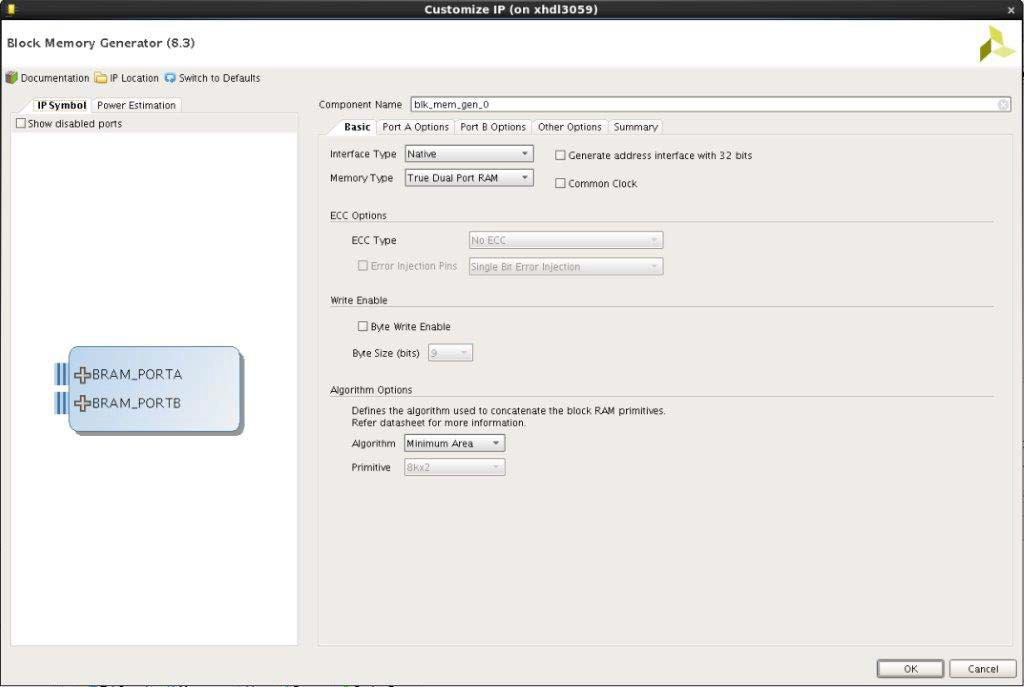
\includegraphics[width=0.6\textwidth]{3}
\caption{Рис.3}
\label{3_label}
\end{figure}

В стартовой диалоговой панели \emph {мастера}, вид которой показан на рисунке, указывается тип создаваемого элемента памяти, его название, а также алгоритм его реализации. 
\begin{itemize}
\item Название формируемого вида запоминающего устройства вводится с помощью клавиатуры в поле редактирования Component Name.
\end{itemize}

На выбор доступны два типа интерфейса – Native и AXI4.

Память блоков интерфейса AXI4 построена на памяти блоков нативного (Native) типа. Доступны два стиля интерфейса AXI4: AXI4 и AXI4-Lite. Также на выбор конфигурируется ядро. Далее на выбор предполагается настройка устройства памяти как ведомое или периферийно. В дополнение к приложениям, поддерживаемым нативным интерфейсом, AXI4 может также использоваться в приложениях AXI4 System Bus и приложениях типа Point-to-Point.

Для нативного типа интерфейса предполагаются следующие параметры настройки:

\begin{itemize}
\item Для определения типа генерируемого элемента памяти следует воспользоваться группой кнопок с зависимой фиксацией Memory Type. Если в нажатом состоянии зафиксирована кнопка Single Port RAM, то будет сформировано ОЗУ с одним портом записи и одним портом чтения данных. При нажатой кнопке Simple Dual Port RAM создается элемент двухпортовой оперативной памяти с одним портом чтения данных.Кроме того, при выборе данного типа памяти становится доступной опция ECC (Error Correction Checking) Type, созданная для регистрации и исправления ошибок с помощью кода Хэмминга и поиска необходимых совместимостей. Для генерации ОЗУ с двумя портами чтения и двумя портами записи данных нужно переключить в нажатое состояние кнопку True Dual Port RAM. Формирование однопортового постоянного запоминающего устройства осуществляется при нажатой кнопке Single Port ROM. Чтобы создать элемент двухпортовой постоянной памяти, следует перевести во включенное состояние кнопку Dual Port ROM. Для двухпортовых элементов доступна опция Common Clock для синхронизации часов ввода (управление одним буфером)
\item Также может быть установлен режим побайтной записи. Для этого нужно перевести в состояние \emph {включено} индикатор Use Byte Write Enable, который расположен во встроенной панели Write Enable.
\item Побайтная запись может осуществляться с контролем и без контроля четности. При этом размер записываемого байта (количество бит в байте) зависит от использования контроля четности. В случае отсутствия контроля четности длина байта составляет восемь бит. Чтобы побайтная запись выполнялась с контролем четности, в состав байта данных должно входить девять бит (восемь бит данных и один контрольный). 
\item Размер байта (и, соответственно, использование контроля четности) указывается с помощью поля выбора Byte Size.
\item Запоминающее устройство, генерируемое с помощью параметризированного модуля Block Memory Generator, строится в виде совокупности примитивов блочной памяти Block RAM primitive. В общем случае каждый из используемых примитивов может иметь различную организацию. Количество и состав возможных вариантов организации примитивов блочной памяти Block RAM primitive определяется выбранным семейством ПЛИС. Тип организации примитивов блочной памяти и алгоритм их соединения для получения запоминающего устройства с требуемой емкостью и организацией указывается с помощью двух кнопок с зависимой фиксацией, которые расположены во встроенной панели Algorithm. Когда в нажатом состоянии находится кнопка Minimum Area, создаваемый элемент памяти составляется из примитивов с различной организацией с целью минимизации используемого количества модулей блочной памяти Block RAM кристалла ПЛИС. При нажатой кнопке Low Power создаваемый элемент памяти будет состоять из тех же, модулей, что и в Minimum Area ядре, но включёнными только при записи или чтении. При нажатой кнопке Fixed Primitive для построения требуемого запоминающего устройства будут использоваться примитивы блочной памяти одного типа, организация которого указывается пользователем с помощью поля выбора Primitive. Содержимое выпадающего списка этого поля выбора зависит от семейства ПЛИС, для которого создается элемент памяти.
\end{itemize}


\subsubsection{Port A|B options}

Вторая диалоговая панель \emph{мастера} настройки параметров генератора оперативных и постоянных запоминающих устройств, реализуемых на основе блочной памяти ПЛИС, предназначена для определения емкости формируемого элемента памяти, а также описания организации и режима работы первого (или единственного) порта запоминающего устройства. 

\begin{figure}[h]
\centering
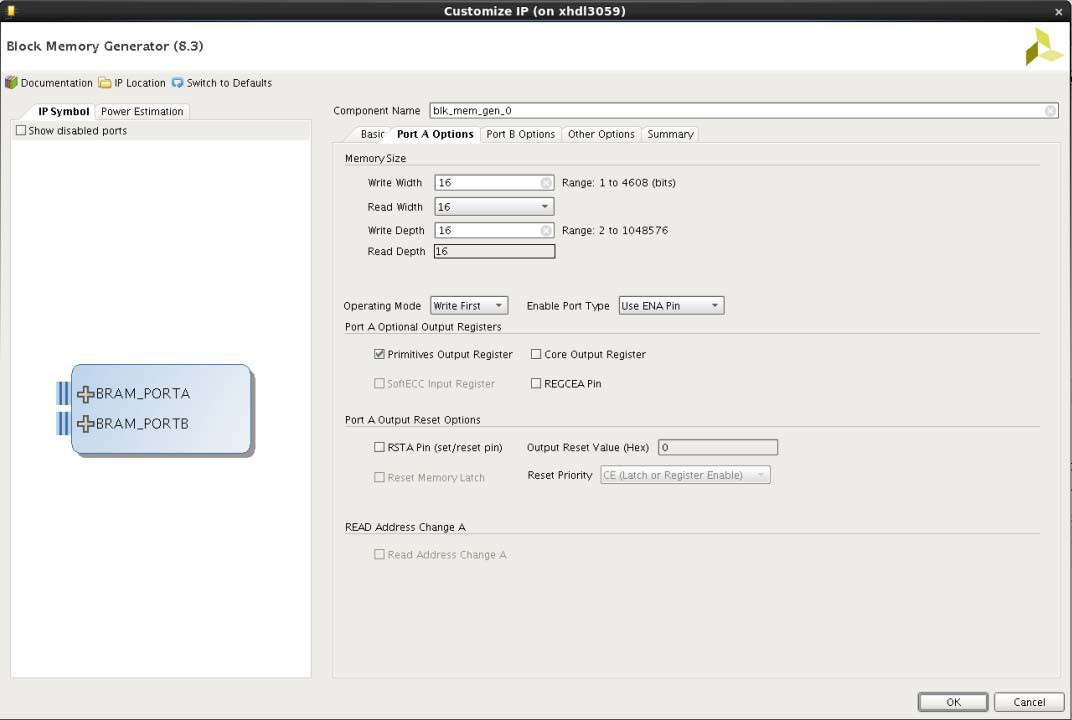
\includegraphics[width=0.6\textwidth]{4}
\caption{Рис.4}
\label{4_label}
\end{figure}

\begin{itemize}
\item Чтобы указать информационную емкость формируемого элемента памяти и разрядность первого (или единственного) порта записи и чтения данных, нужно воспользоваться полями редактирования и выбора, расположенными во встроенной панели Memory Size. Прежде всего, рекомендуется определить разрядность первого входного порта Port A, предназначенного для записи данных, с помощью поля редактирования Write Width. Требуемое число разрядов этого порта (в диапазоне от 1 до 1152) указывается с помощью клавиатуры, после активизации данного поля редактирования. Количество ячеек памяти в формируемом запоминающем устройстве задается в поле редактирования Write Depth. Максимальное значение этого параметра ограничено объемом физических ресурсов блочной памяти Block RAM используемого кристалла ПЛИС. Таким образом, информационная емкость создаваемого элемента памяти, выраженная в битах, равна произведению значений параметров Write Width и Write Depth. Разрядность первого (или единственного) выходного порта, используемого для чтения данных из памяти, определяется с помощью поля выбора Read Width. Выпадающий список этого поля выбора содержит допустимые варианты разрядности первого выходного порта, которые соответствуют установленному значению разрядности первого входного порта записи данных. Количество разрядов адреса (адресных входов) в формируемом запоминающем устройстве вычисляется автоматически, исходя из установленных значений параметров, рассмотренных выше. Значения параметров Write Width и Read Width должны быть кратны размеру байта данных, указанному в поле выбора Byte Size. В этом случае вместо обычного (одиночного) входа разрешения записи данных используется шина, количество разрядов которой вычисляется автоматически в соответствии с указанным значением разрядности порта записи. 
\item Для определения режима работы первого (или единственного) выходного порта элемента оперативной памяти, предназначенного для чтения данных, при выполнении операции записи данных в ОЗУ нужно воспользоваться группой кнопок с зависимой фиксацией Operating Mode. Если в нажатом состоянии находится кнопка Write First, то данные, поступающие во входной порт, записываются в соответствующую ячейку памяти (адрес которой задается комбинацией сигналов на адресных входах), после чего сразу передаются на выходы запоминающего устройства. При нажатии кнопки Read First в генерируемом элементе оперативной памяти будет установлен режим предварительного чтения данных из указанной ячейки перед записью новых данных в эту ячейку. Таким образом, при осуществлении операции записи данных, поступающих во входной порт формируемого элемента ОЗУ, на его выходах будет отображаться информация, которая содержалась в соответствующей ячейке перед этим (на предыдущем такте). Когда в нажатое состояние переводится кнопка No Change, в формируемом элементе ОЗУ будет установлен режим блокировки выходов при выполнении операции записи данных. В этом режиме на протяжении всего цикла записи выходы находятся в зафиксированном состоянии, которое соответствует последним считанным данным, присутствовавшим в момент переключения сигнала разрешения записи в активное состояние. 
\item Чтобы сформировать элемент запоминающего устройства с входом разрешения операций для первого порта, нужно переключить в нажатое состояние кнопку Use ENA Pin. При этом в созданном элементе памяти выполнение операций записи и чтения данных для первого порта будет возможно только при активном уровне сигнала на входе разрешения ENA.
\item Для определения состояния выходного регистра или защелки формируемого запоминающего устройства в режиме сброса (или установки) следует воспользоваться полем редактирования Output Reset Value (Hex), которое расположено во встроенной панели Output Reset. Значение, указываемое в этом поле редактирования, должно быть представлено в шестнадцатеричном формате. При этом количество шестнадцатеричных символов должно соответствовать разрядности первого порта чтения данных. Чтобы задействовать в формируемом элементе памяти вход синхронного сброса (или установки) для первого порта (Port A), следует установить индикатор Use SSRA Pin, находящийся в этой же встроенной панели, в состояние \emph {включено}. 
\item Если в стартовой диалоговой панели \emph {мастера} настройки параметров генератора элементов памяти был выбран двухпортовый тип запоминающего устройства, то третья диалоговая панель будет позволять определить основные параметры второго порта (Port B) создаваемого элемента памяти. Все параметры этого порта, за исключением разрядности, указываются так же, как и для первого порта (Port A). Количество разрядов второго порта записи данных не может быть установлено произвольно. Значение этого параметра должно быть кратным числу разрядов первого порта записи данных (с фиксированным набором коэффициентов кратности), которое было указано в диалоговой панели, представленной на рисунке. Поэтому разрядность второго порта записи данных задается с помощью поля выбора Write Width, выпадающий список которого содержит только допустимые значения данного параметра. Содержимое этого списка автоматически корректируется при изменении значения разрядности первого порта записи данных. 
\end{itemize}

\subsubsection{Other options}

Предпоследняя диалоговая панель \emph {мастера} настройки параметров генератора оперативных и постоянных запоминающих устройств, реализуемых на основе блочной памяти ПЛИС, позволяет выбрать тип и конфигурацию выходных регистров, а также указать параметры инициализации формируемого элемента памяти. 

\begin{figure}[h]
\centering
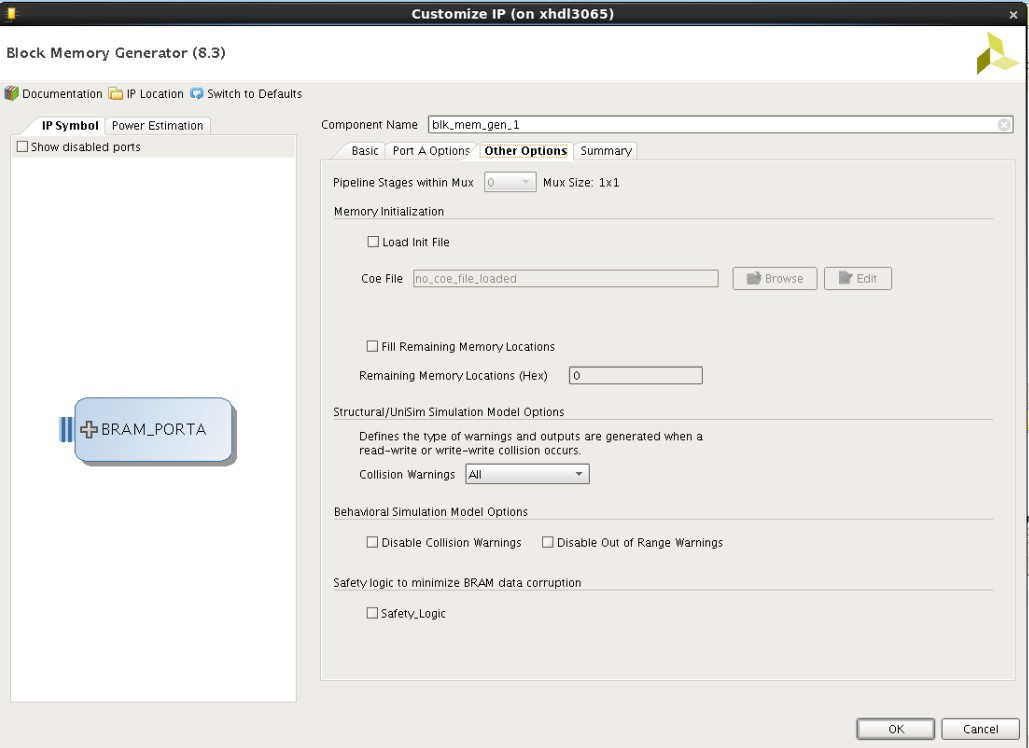
\includegraphics[width=0.6\textwidth]{5}
\caption{Рис.5}
\label{5_label}
\end{figure}

\begin{itemize}
\item Стадии конвейера в пределах Мультиплексора: доступна только, когда опция Register Output of Memory Core выбрана и для порта A и для порта B и когда у созданной памяти есть больше чем один примитив (так, чтобы MUX был необходим при выводе). Выберите значение 0, 1, 2, или 3 из выпадающего списка.
\item Для автоматической инициализации содержимого генерируемых запоминающих устройств, реализуемых на основе блочной памяти ПЛИС, следует определить значения соответствующих параметров с помощью элементов управления, которые расположены во встроенной панели Memory Initialization. Информацию, которую нужно записать в соответствующие ячейки формируемого элемента памяти, можно указать в виде файла формата COE. Для этого нужно, прежде всего, переключить индикатор Load Init File в состояние «включено», после чего станут доступными поле редактирования COE File и кнопка Browse. При нажатии на данную кнопку на экран выводится стандартная панель диалога открытия файла, с помощью которой нужно найти на одном из дисков компьютера требуемый файл, описывающий содержимое создаваемого запоминающего устройства. После выбора соответствующего файла и закрытия стандартной диалоговой панели его название автоматически отображается в поле редактирования COE File. Можно также с помощью клавиатуры сразу указать в этом поле редактирования название требуемого файла инициализации, не выполняя процедуру его поиска. Для быстрого просмотра содержимого выбранного файла нужно воспользоваться кнопкой Show, которая находится во встроенной панели Memory Initialization. Если указываемый файл инициализации описывает содержимое только части генерируемого запоминающего устройства, то все оставшиеся неинициализированными ячейки памяти могут быть заполнены по умолчанию значением, определяемым пользователем. С этой целью нужно установить индикатор Fill Remaining Memory Locations в состояние \emph {включено}. При этом становится доступным поле редактирования Remaining Memory Locations (Hex), в котором нужно с помощью клавиатуры указать шестнадцатеричное значение, записываемое по умолчанию в ячейки памяти, оставшиеся неопределенными. Количество шестнадцатеричных символов, указываемых в этом поле редактирования, должно соответствовать разрядности первого порта записи генерируемого запоминающего устройства. 
\item Structural/UNISIM Simulation Model Options: Выберите тип предупреждающих сообщений и выводов, сгенерированных структурной моделью моделирования в случае коллизий. Для опций ALL, WARNING ONLY и GENERATE X ONLY, обнаружения коллизий, опция активирована в моделях UNISIM, чтобы обработать коллизию при любом условии.
\item Behavioral Simulation Model Options: Выберите тип предупреждающих сообщений, сгенерированных моделью моделирования на поведенческом уровне. Выберите, должна ли модель принять синхронные часы (Общие Часы) для предупреждений коллизии.
\item Dynamic Power Saving: экономия электроэнергии включена в положении, когда память активно не используется в течение длительного периода времени. Если матрица элементов памяти входит в режим ожидания, данные сохраняются. Чтобы использовать память, установите контакт сна в 0.
\end{itemize}

\subsubsection{Summary}

Заключительная диалоговая панель \emph {мастера} настройки генератора оперативных и постоянных запоминающих устройств, реализуемых на основе блочной памяти ПЛИС, отражает параметры создаваемого устройства в виде списка.

\begin{figure}[h]
\centering
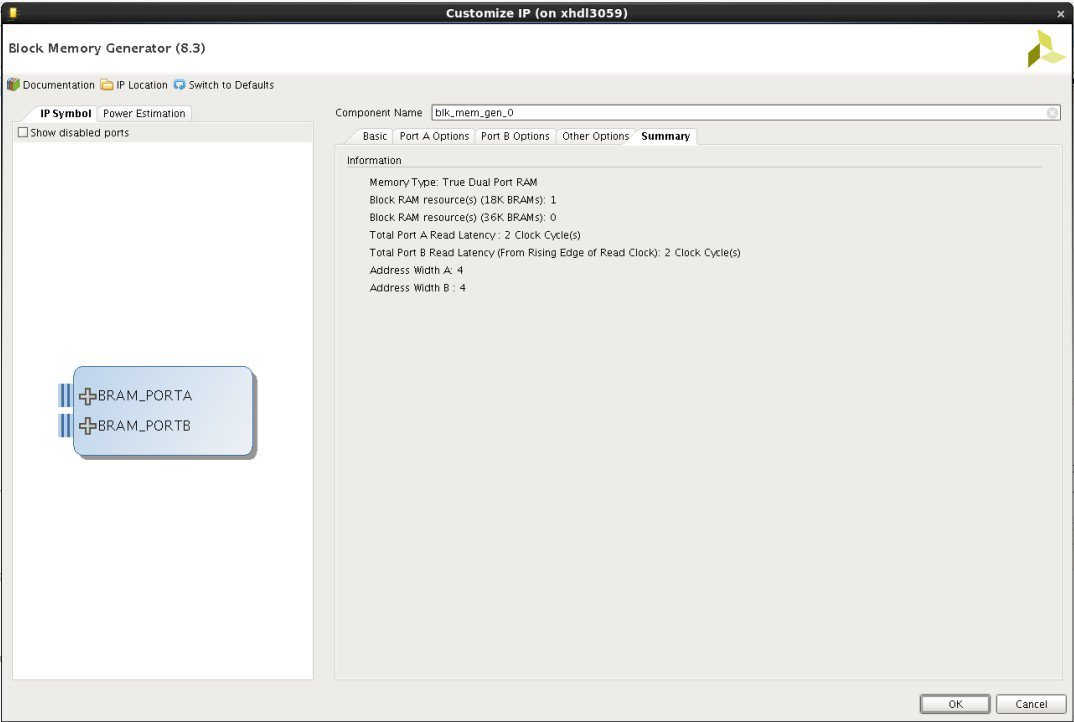
\includegraphics[width=0.6\textwidth]{6}
\caption{Рис.6}
\label{6_label}
\end{figure}

\begin{itemize}
\item Memory Type: Сообщает о выбранном типе памяти.
\item Block RAM Resources: Сообщает точный номер 18 K и 36 K блочных примитивов RAM, которые используются, чтобы создать ядро.
\item Total Port A Read Latency: номер тактов для Операции чтения для порта A. Этим значением управляют дополнительные выходные опции регистров для порта на предыдущей вкладке.
\item Total Port B Read Latency: номер тактов для Операции чтения для порта B. Этим значением управляют дополнительные выходные опции регистров для порта B на предыдущей вкладке.
\item Address Width: фактическая ширина адресной шины к каждому порту.
\end{itemize}

\subsubsection{Power Estimation}

\begin{figure}[h]
\centering
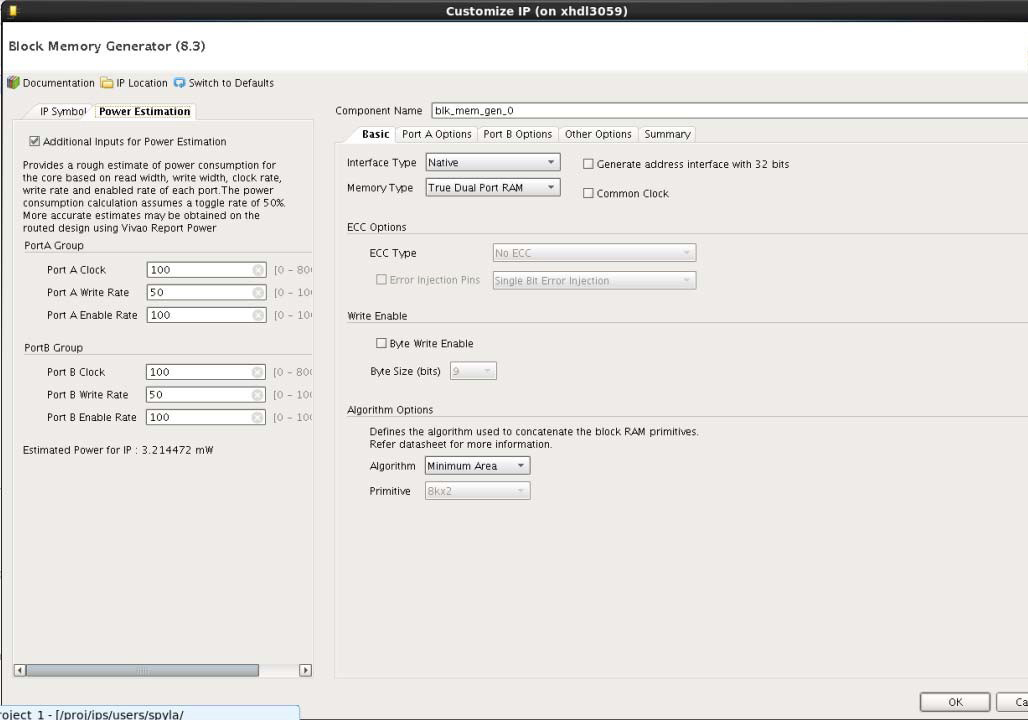
\includegraphics[width=0.6\textwidth]{7}
\caption{Рис.7}
\label{7_label}
\end{figure}

Вкладка Power Estimation на левой стороне IDE Vivado, показанная на рисунке, обеспечивает грубую оценку потребляемой мощности для ядра, основанного на сконфигурированных параметрах Read width, Write width, clock rate, Write rate and enable rate для каждого порта.
 
У этой вкладки есть опция  \emph {Additional Inputs for Power Estimation}, созданная для ввода дополнительных оценок потребляемой мощности. Можно ввести следующие параметры для расчета питания: Clock Frequency [A|B] (тактовая частота портов А и В), Write Rate [A|B] (скорость записи для портов А и В), Enable Rate [A|B] (средняя скорость доступа к портам А и В)

\subsection{Включение созданного ядра в код VHDL}

После выбора необходимых параметров для модуля BRAM следует нажать OK, a затем Generate во всплывающем окне. После того, как завершится синтез нашего модуля, переходим на вкладку IP Sources и открываем Файл в формате .vho в папке Instantiation Template(см. Рис. 8)

\begin{figure}[h]
\centering
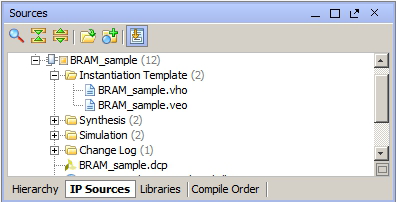
\includegraphics[width=0.6\textwidth]{8}
\caption{Рис. 8}
\label{8_label}
\end{figure}

В этом файле уже созданы вставки для определения компонента в основном коде и инстанциация для тестбенча (рис. 9-10)

\begin{figure}[h]
\centering
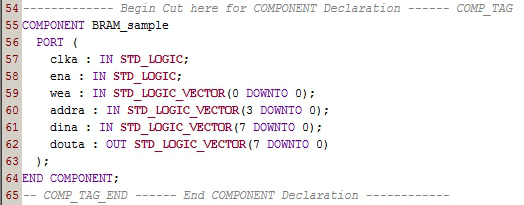
\includegraphics[width=0.6\textwidth]{9}
\caption{Рис. 9}
\label{9_label}
\end{figure}

\begin{figure}[h]
\centering
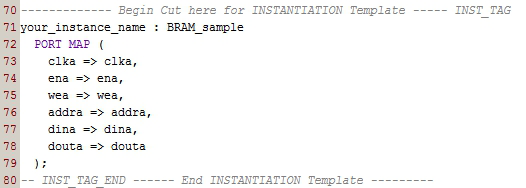
\includegraphics[width=0.6\textwidth]{10}
\caption{Рис. 10}
\label{10_label}
\end{figure}

\subsection{Симуляция}

В качестве примера рассмотрим BRAM со следующими параметрами (всё, что не указано ~-- по умолчанию):
\begin{enumerate}
%\item Component Name: BRAM_sample, Algorithm: Low Power
\item Algorithm: Low Power
\item Write width:8, Read width:8, Write depth:16
\item Галочка Fill Remaining memory locations
\end{enumerate}

Напишем тестбенч для данного модуля памяти: 

\lstinputlisting[caption=Тестбенч, label=09-bram]{proga1.vhd}

Результаты симуляции:

\begin{figure}[h]
\centering
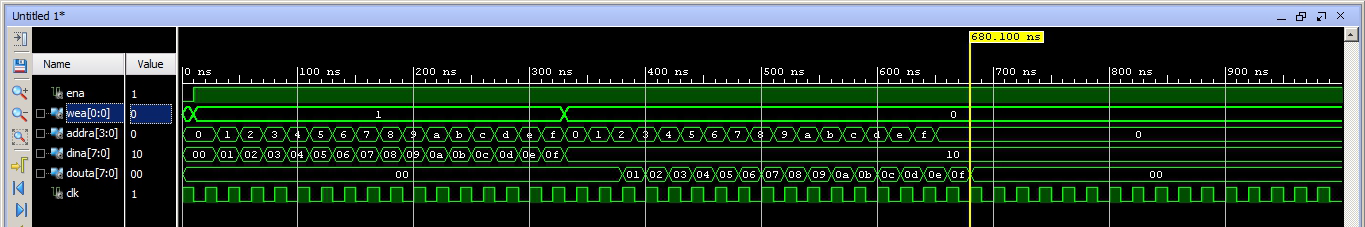
\includegraphics[width=0.6\textwidth]{11}
\caption{Рис. 11}
\label{11_label}
\end{figure}

\section{Лабораторная работа: Накопитель памяти на основе BRAM}

Задача: написать VHDL-код накопителя, использующего BRAM. Накопитель имеет вход $data(din)$ и вход $valid(dv_in)$, в накопитель поступают данные с паузами; затем, когда поступило N (16) отсчетов данных, буфер выдает последовательно без пауз все пришедшие ранее отсчеты данных.

\subsection{Создаём модуль BRAM}
\subsection{Реализация на VHDL}

\lstinputlisting[caption=Реализация кода, label=09-bram]{proga2.vhd}

\subsection{Самопроверяющийся тестбенч}

\lstinputlisting[caption=Тестбенч, label=09-bram]{proga3.vhd}